\documentclass[12pt, a4papre]{article}
\usepackage[catalan]{babel}
\usepackage[unicode]{hyperref}
\usepackage{amsmath}
\usepackage{amssymb}
\usepackage{amsthm}
\usepackage{xifthen}
\usepackage{listings}
\usepackage{float}
\usepackage{siunitx}
\usepackage{graphicx}
\usepackage{indentfirst}
\usepackage{tikz} 

\newcommand{\norm}[1]{\lvert #1 \rvert}

\hypersetup{
    colorlinks = true,
    linkcolor = blue
}

\author{Elexioma de l'acció}
\title{10. Torre de $\pi$sa}
\date{}

\begin{document}
	\maketitle

	L'Anna, amb gran curiositat es preguntava quina era la probabilitat de creuar el riu, i com a molt bona matematica que era, va veure que totes les combinacions eren equiprobables, al ser els ponts existents amb una probabilitat de $\frac{1}{2}$. Així doncs va arribar a la conclusió que la probabilitat de poguer creuar el pont era la de casos probables entre casos possibles. Va demanar doncs a un estadistic molt treballador que resolgues de la forma mes inteligent possible el problema. Just quan aquest estava a punt d'acabar la resolució el estadistic a l'Anna se li va acudir una resolució alternativa molt mes maca. Presentem aquí les 2 ressolucions, la de l'Anna i la del estadistic.
	
	\begin{proof} Podem reduir al problema a si existeix un cami entre els nodes 0 i 7 del següent graph.
	
\begin{center}
\begin{tikzpicture}[node distance={15mm}, thick, main/.style = {draw, circle}]
\node[main] (1) {0}; 
\node[main] (2) [above right of=1] {3}; 
\node[main] (3) [right of=1] {2}; 
\node[main] (4) [below right of=1] {1}; 
\node[main] (5) [right of=2] {6}; 
\node[main] (6) [right of=3] {5}; 
\node[main] (7) [right of=4] {4}; 
\node[main] (8) [right of=6] {7};
\draw (1) -- (2); 
\draw (1) -- (3); 
\draw (1) -- (4); 
\draw (2) -- (3); 
\draw (3) -- (4); 
\draw (2) -- (5); 
\draw (3) -- (6); 
\draw (4) -- (7); 
\draw (5) -- (6); 
\draw (6) -- (7); 
\draw (5) -- (8); 
\draw (6) -- (8); 
\draw (7) -- (8); \end{tikzpicture} 
\end{center}

		Apuntem ara que el cami no existeix si existeix un tall de baix cap a dalt que fa que tant el node 0 com el node 7 estiguin a 2 components conexes diferents. Si estan en dos components conexes diferents existeix un cami entre ponts trencats per on es pot passar d'un canto a l'altre del pont per dins del riu (sense passar per sota de cap pont). Considerem el següents 2 graphs.
		
		\begin{figure}[H]
		        \begin{center}
		        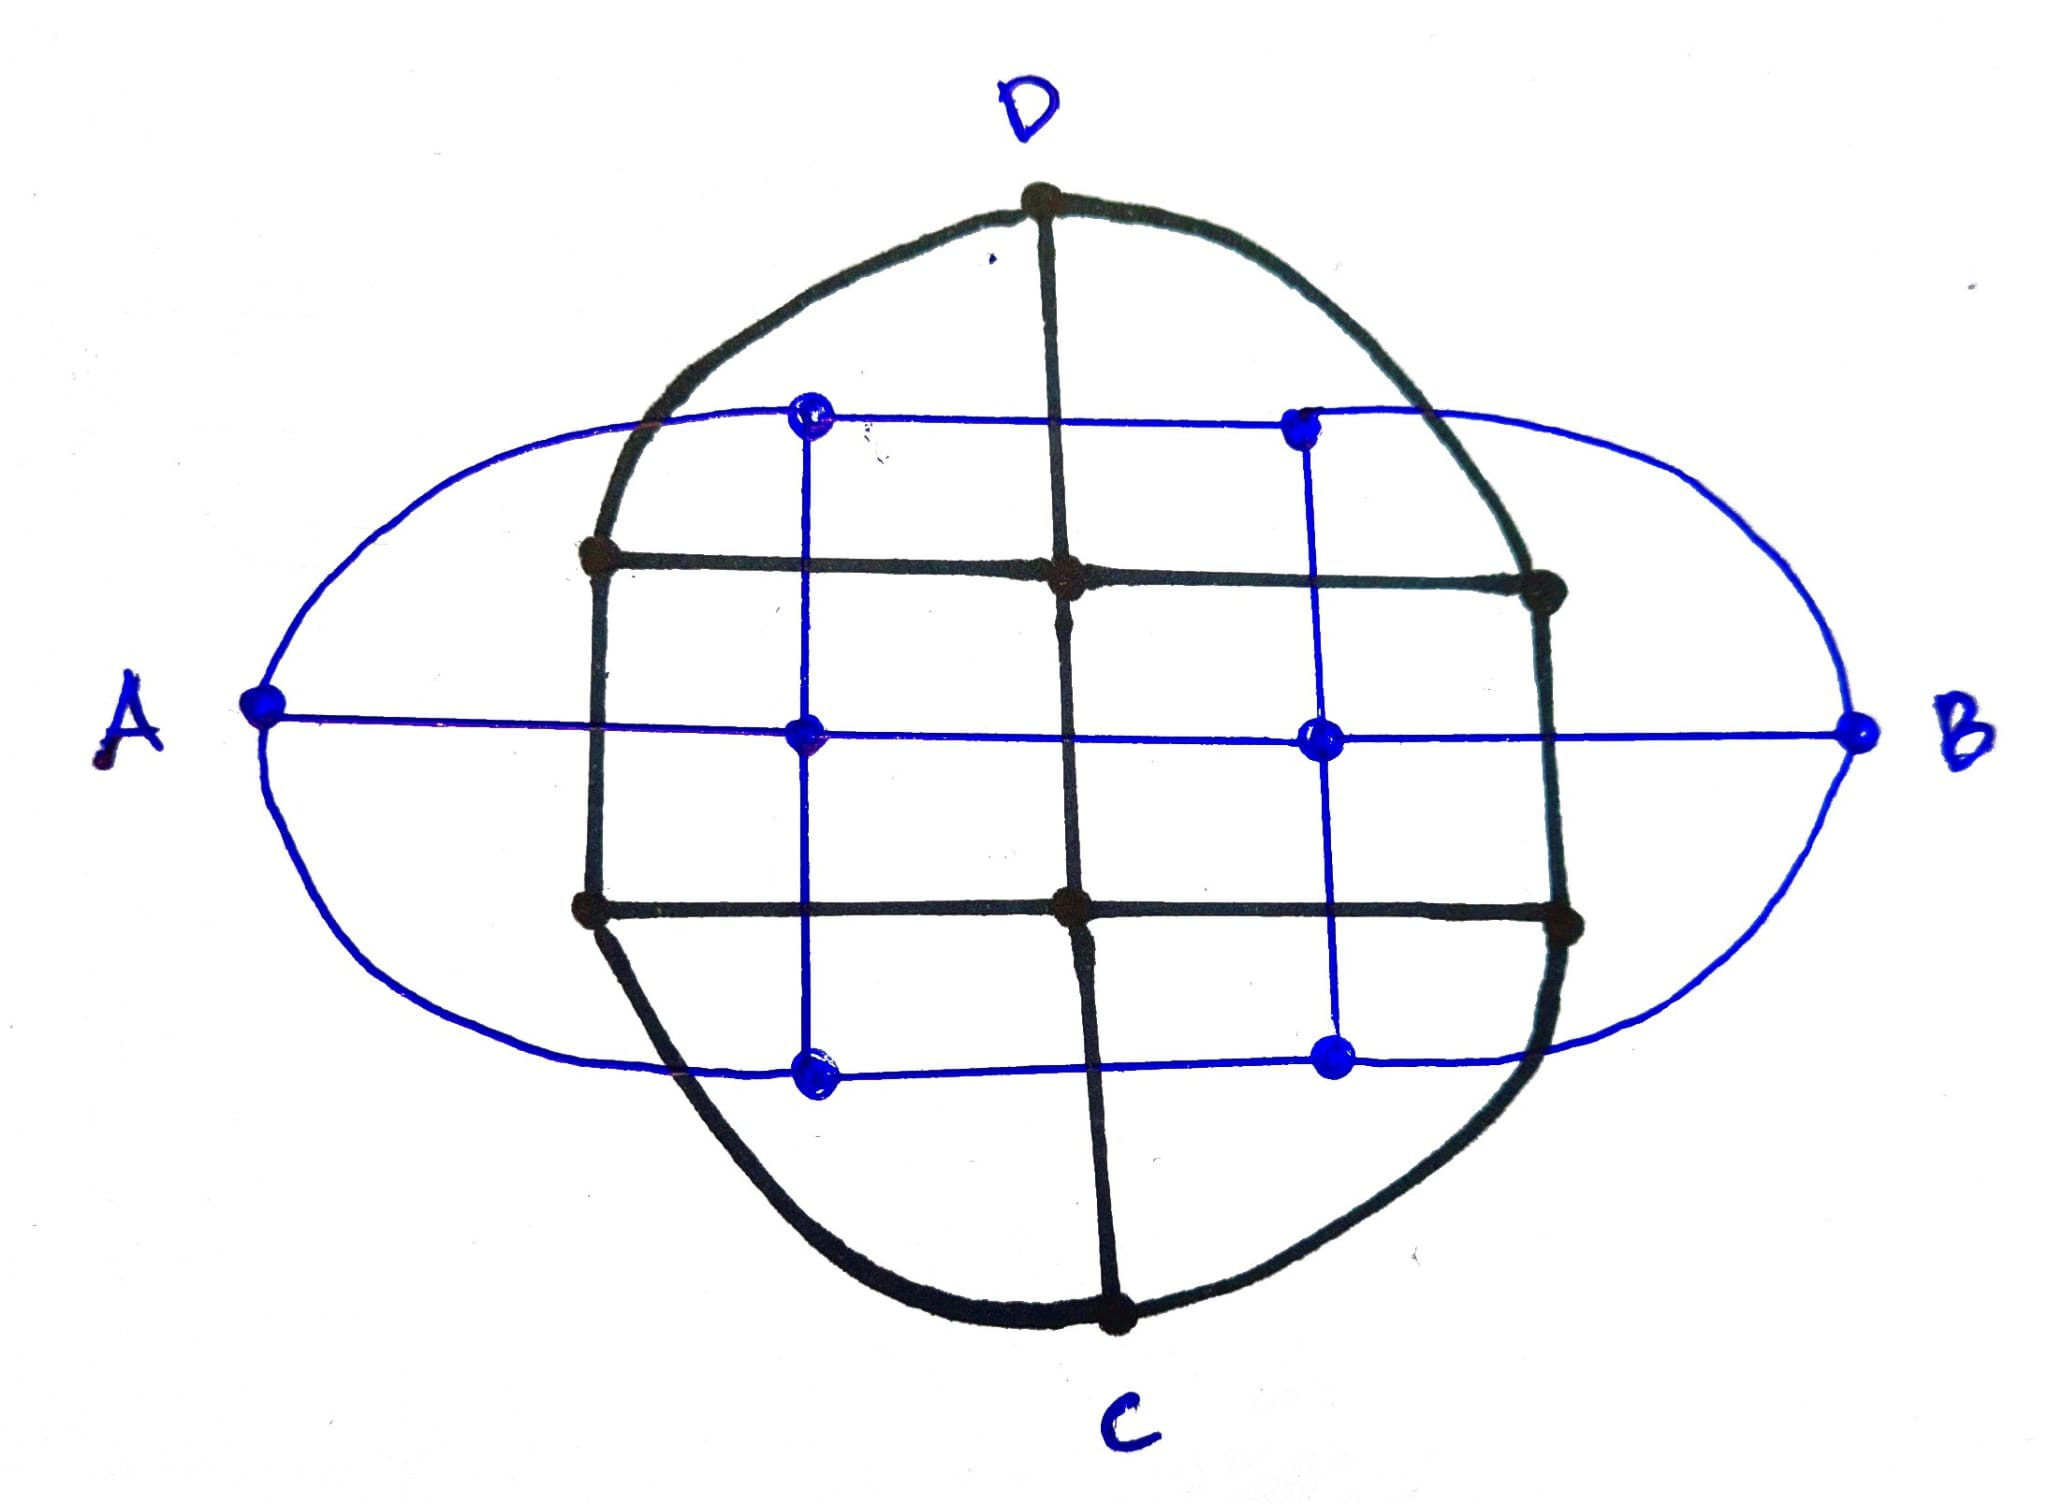
\includegraphics[width=80mm]{graph2}
		        \caption{Simulació 3.6}
		        \end{center}
		    \end{figure}
		\graphicspath{ {./Images/} }
		
		Si no es pot anar de A fins a B, aleshores es podra anar de C fins a D per algun cami sense creuar cap pont. Per tant podem considerar el graph negre com el complementari al graph blau un cop trencat. Veiem també que si es pot anar d'A fins a B aleshores no es podrà anar de C fins a D sense creuar cap pont. Així doncs, per simetria podem concloure que l'Anna podrà creuar el pont amb una probabilitat de $\frac{1}{2}$, al ser el graph blau i negre iguals i tenir les mateixes condicions per a poder d'anar d'A fins a B i de C fins a D respectivament.
		
	\end{proof}
	
	

	
	
\end{document}